\documentclass[12pt,t]{beamer}
 
\usepackage[utf8]{inputenc} 
\usepackage[T1]{fontenc}
\usepackage{lmodern}
\usepackage{graphicx}
\usepackage[english]{babel}
\usepackage[absolute,overlay]{textpos}
\usepackage{epstopdf}
\usepackage{tikz}
\usetikzlibrary{shapes}
 
\usetheme{PaloAlto}

\usefonttheme{professionalfonts}
\usefonttheme{serif}

\setbeamercolor{footline}{fg=blue}
\setbeamerfont{footline}{series=\bfseries}

\addtobeamertemplate{navigation symbols}{}{%
    \usebeamerfont{footline}%
    \usebeamercolor[fg]{footline}%
    \hspace{1em}%
    \insertframenumber/\inserttotalframenumber
}

\title[Notes]{Notes}
\author[F.Ardiani, A.A. Manelli, C.J. Ruestes, C.A. Careglio, E.M. Bringa]{Franco Ardiani$^a$, Andrés A. Manelli$^a$, Carlos J. Ruestes$^b$, Claudio A. Careglio$^{a,c}$ and Eduardo M. Bringa$^{b,d}$}
\institute[UNCUYO]{$^a$Facultad de Ingeniería, Universidad Nacional de Cuyo\\$^b$ITIC, Universidad Nacional de Cuyo\\$^c$FCEN, Universidad Nacional de Cuyo\\$^d$CONICET}
\date{\today}


\begin{document}

\section{Introduction notes}

\begin{frame}
   \frametitle{Contents}
   \tableofcontents[currentsection,sectionstyle=show/shaded,subsectionstyle=show/shaded/hide]
\end{frame}

\begin{frame}
\frametitle{Introduction notes}
 \begin{textblock*}{10.6cm}(1.8cm,2cm) 
\begin{itemize}
  \item Example applications for MGs: amorphous structural steels, biomedical materials, aerospace materials, etc.
  \item Production of MGs: techniques which include high quenching rates, low volumes and composition control.
  \item STZs and SBs: STZs are small zones of intense shearing strain, consisting of a few atoms. A SB contains more atoms and has a different aspect ratio.
  \item Porosity to evitate the propagation of SBs: related to the way of preventing dislocation motion in metals.
 \item MD (Molecular Dynamics): solves problems with many bodies by applying an atom to atom potential.
\end{itemize} 
\end{textblock*}
\end{frame}

\section{Simulation details notes}

\begin{frame}
\frametitle{Simulation details notes}
\vspace{-0.3cm}
 \begin{textblock*}{10.6cm}(1.8cm,4.5cm) 
\begin{itemize}
 \item EAM: the total energy $E_i$ of an atom $i$ is given by this equation, where F is the embedding energy which is a function of the atomic electron density $\rho$, $\phi$ is a pair potential interaction, and $\alpha$ and $\beta$ are the element types of atoms I and J. The multi-body nature of the EAM potential is a result of the embedding energy term. Both summations in the formula are over all neighbors J of atom I within the cutoff distance.
\end{itemize}
\end{textblock*}
	\begin{exampleblock}{EAM}
	\[
		E_i=F_{\alpha} \left ( \sum \limits_{i\neq j} \rho _{\beta} (r_{ij}) \right ) + \frac{1}{2} \sum \limits_{i\neq j} \phi _{\alpha \beta} (r_{ij})
	\]
	\end{exampleblock}
\end{frame}

\begin{frame}
\frametitle{Simulation details notes}
\vspace{-0.3cm}
 \begin{textblock*}{10.6cm}(1.8cm,4.5cm) 
\begin{itemize}
 \item EAM: the potential energy of an atom, $i$, is given by this equation, where $r_{ij}$ is the distance between atoms $i$ and $j$, $\phi_{\alpha\beta}$ is a pair-wise potential function, $\rho_\beta$ is the contribution to the electron charge density from atom $j$ of type $\beta$ at the location of atom $i$, and $F$ is an embedding function that represents the energy required to place atom $i$ of type $\alpha$ into the electron cloud.
\end{itemize}
\end{textblock*}
	\begin{exampleblock}{EAM}
	\[
		E_i=F_{\alpha} \left ( \sum \limits_{i\neq j} \rho _{\beta} (r_{ij}) \right ) + \frac{1}{2} \sum \limits_{i\neq j} \phi _{\alpha \beta} (r_{ij})
	\]
	\end{exampleblock}
\end{frame}


\section{Results notes}

\subsection{Compression}

\begin{frame}
\frametitle{Compression}
\framesubtitle{Other plots}
  \begin{textblock*}{6.5cm}(2.5cm,2cm) % {block width} (coords)
  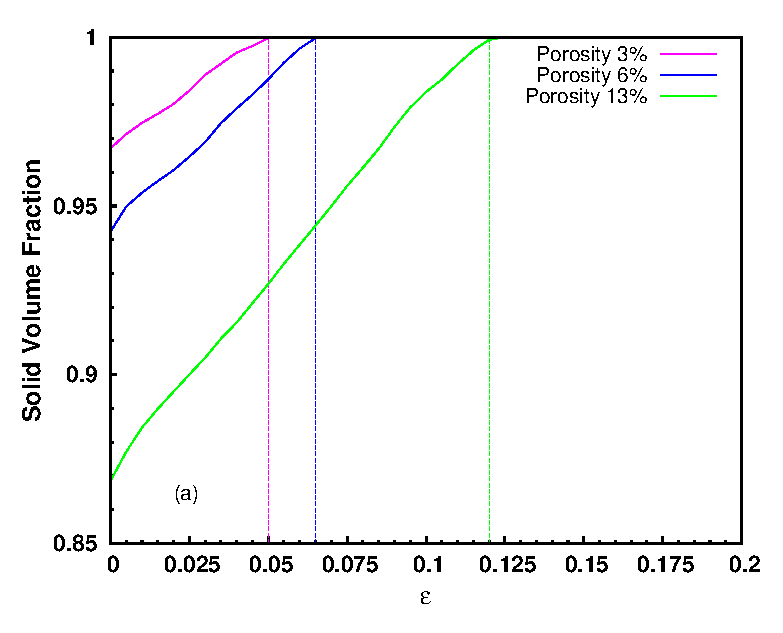
\includegraphics[width=6.5cm]{SVF_strain_comp_dash.eps}
  \end{textblock*}
\begin{textblock*}{3cm}(9.2cm,2.5cm) % {block width} (coords)
  Solid volume fraction versus strain.
\end{textblock*}
\begin{textblock*}{9cm}(2.8cm,7.4cm) % {block width} (coords)
  The dashed lines show when pores totally close. The values are: \\
  $3\% \rightarrow 0.05, 6\% \rightarrow 0.065, 13\% \rightarrow 0.12$
\end{textblock*}
\end{frame}

\begin{frame}
\frametitle{Compression}
\framesubtitle{Other plots}
  \begin{textblock*}{6.5cm}(2.5cm,2cm) % {block width} (coords)
  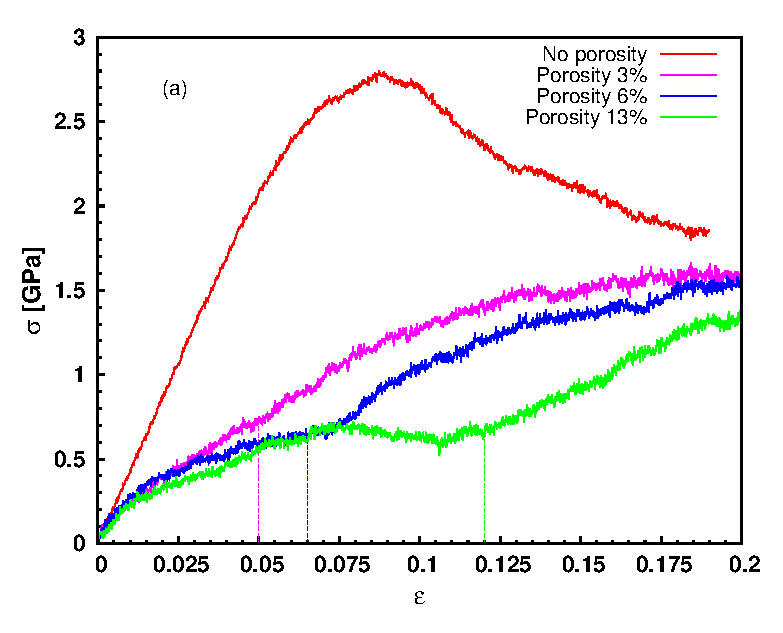
\includegraphics[width=6.5cm]{stress_strain_comp_dash.eps}
  \end{textblock*}
\begin{textblock*}{3cm}(9.2cm,2.5cm) % {block width} (coords)
  Von Mises stress versus strain.
\end{textblock*}
\begin{textblock*}{9cm}(2.8cm,7.8cm) % {block width} (coords)
  We can further appretiate the hardening effect.
\end{textblock*}
\end{frame}


\subsection{Tension}

\begin{frame}
\frametitle{Tension}
\framesubtitle{Other plots}
  \begin{textblock*}{6.5cm}(2.5cm,2cm) % {block width} (coords)
  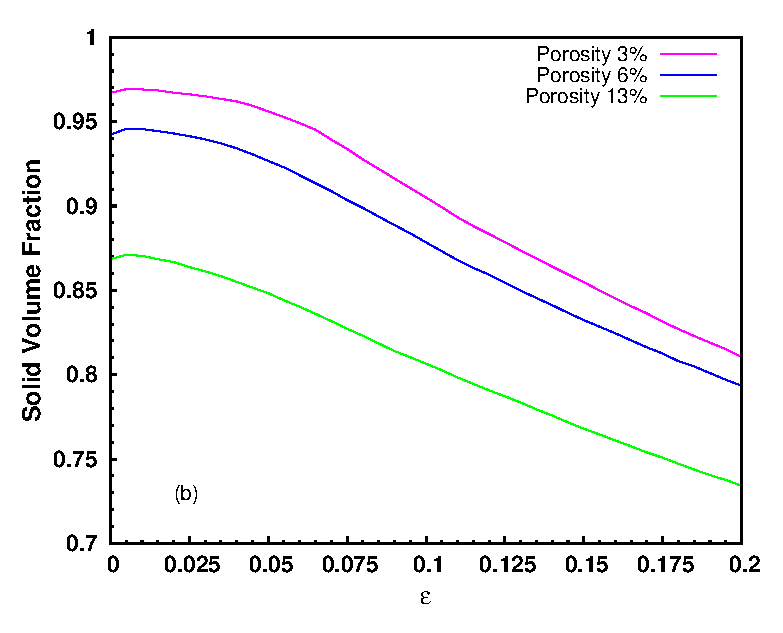
\includegraphics[width=6.5cm]{SVF_strain_tens.eps}
  \end{textblock*}
\begin{textblock*}{3cm}(9.2cm,2.5cm) % {block width} (coords)
  Solid volume fraction versus strain.
\end{textblock*}
\end{frame}

\begin{frame}
\frametitle{Tension}
\framesubtitle{Other plots}
  \begin{textblock*}{6.5cm}(2.5cm,2cm) % {block width} (coords)
  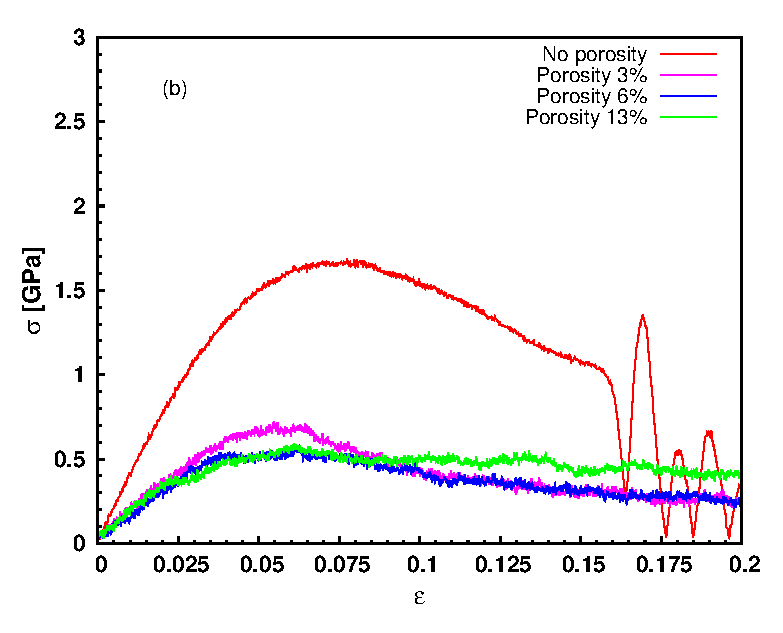
\includegraphics[width=6.5cm]{stress_strain_tens.eps}
  \end{textblock*}
\begin{textblock*}{3cm}(9.2cm,2.5cm) % {block width} (coords)
  Von Mises stress versus strain.
\end{textblock*}
\begin{textblock*}{9cm}(2.8cm,7.8cm) % {block width} (coords)
  We can further appretiate the plastic flow.
\end{textblock*}
\end{frame}

\section{Conclusion notes}

\begin{frame}
\frametitle{Conclusion notes}
\framesubtitle{Comparison with Yuan}
  \begin{textblock*}{5cm}(2cm,3.2cm) % {block width} (coords)
  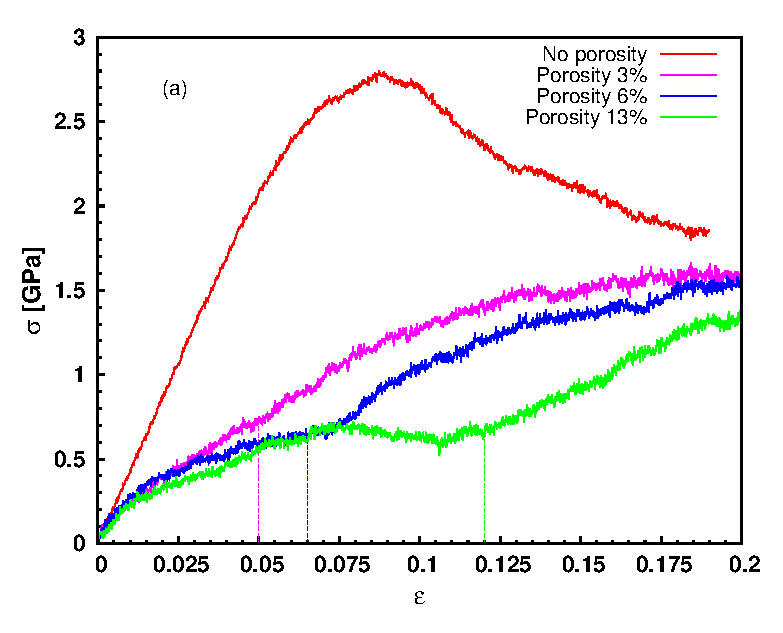
\includegraphics[width=5cm]{stress_strain_comp_dash.eps}
  \end{textblock*}
\begin{textblock*}{3cm}(7cm,3cm) % {block width} (coords)
  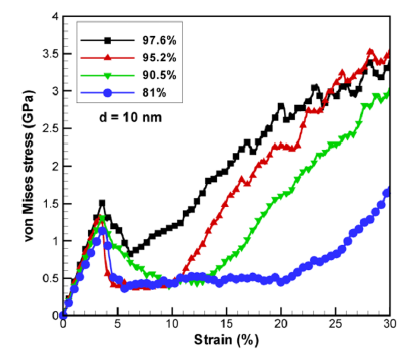
\includegraphics[width=5cm]{Yuan_VM.png}
\end{textblock*}
\begin{textblock*}{12cm}(2.3cm,8.8cm) % {block width} (coords)
\tiny{Yuan F. and Wu X., \textit{AIP ADVANCES}, \textbf{4}, 127109 (2014).}
\end{textblock*}
\end{frame}

\begin{frame}
\frametitle{Conclusion notes}
\framesubtitle{Comparison with Yuan}
  \begin{textblock*}{5cm}(2cm,3.2cm) % {block width} (coords)
  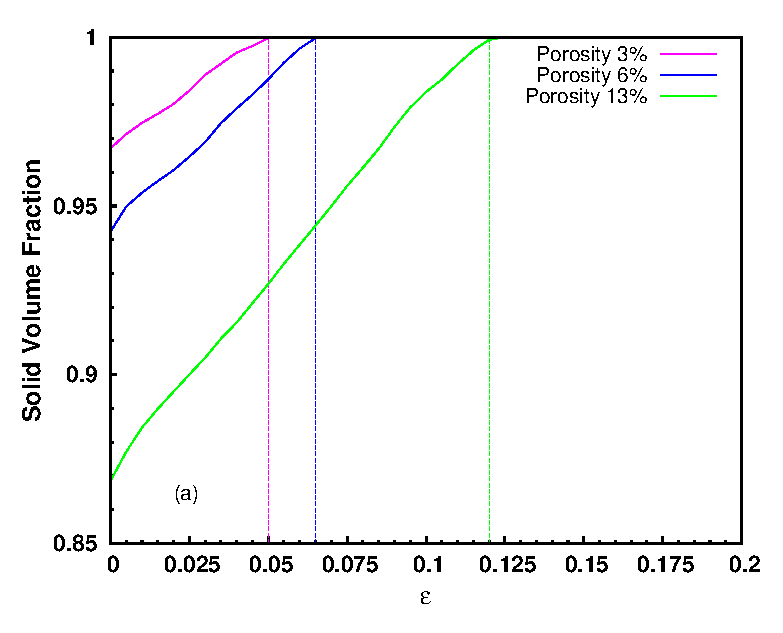
\includegraphics[width=5cm]{SVF_strain_comp_dash.eps}
  \end{textblock*}
\begin{textblock*}{3cm}(7cm,3cm) % {block width} (coords)
  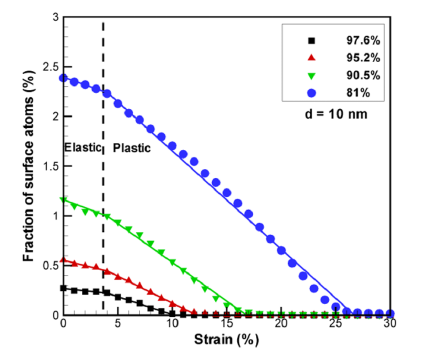
\includegraphics[width=5cm]{Yuan_SVF.png}
\end{textblock*}
\begin{textblock*}{12cm}(2.3cm,8.8cm) % {block width} (coords)
\tiny{Yuan F. and Wu X., \textit{AIP ADVANCES}, \textbf{4}, 127109 (2014).}
\end{textblock*}
\end{frame}

\begingroup
\makeatletter
\setlength{\hoffset}{-.5\beamer@sidebarwidth}
\makeatother
\begin{frame}[plain]
    \maketitle
    \begin{textblock*}{12cm}(2cm,8.5cm) % {block width} (coords)
    \tiny{Acknowledgements:\\ We thank support from SeCTyP-UNCuyo grant B008. EMB and CJR also thank support from PICT-PRH 0092.}
    \end{textblock*}
    \begin{textblock*}{1.5cm}(11.5cm,6.3cm) % {block width} (coords)
    
\includegraphics[width=1.5cm]{fing.png}
    \end{textblock*}
    \begin{textblock*}{2cm}(1.5cm,5.8cm) % {block width} (coords)
    
\includegraphics[width=2cm]{uncuyo.jpg}
    \end{textblock*}
    \begin{textblock*}{2cm}(1.7cm,6.8cm) % {block width} (coords)
    
\includegraphics[width=2cm]{logofcen3.png}
    \end{textblock*}
\end{frame}
\endgroup

\end{document}